% Section 5: Reference Architecture
% Source: context/ICSA_RA_Literature_Review.md §1-8, §12
% Source: context/Paper_Layout_Plan.md §5
%
% EM-DASH PROHIBITION: Do not use --- or \textemdash. Use colons or semicolons.

\section{Reference Architecture}\label{sec:reference_architecture}

\subsection{From Taxonomy to Architectural Requirements}\label{sec:ra_motivation}

The six-outcome taxonomy (Table~\ref{tab:taxonomy}) is not merely a
measurement scheme; each outcome implies a specific architectural requirement.
Character-level corruption (\texttt{corrupted}) requires a reference copy for
verification. Semantic substitution (\texttt{sem\_sub}), where the LLM decodes
the JWT payload and returns a plausible but cryptographically invalid value, is
undetectable by format validation, length checking, or bounded Levenshtein
comparison: the only complete mitigation is to prevent the LLM from processing
the credential at all. Model refusal (\texttt{refusal}) and abstention
(\texttt{abstention}) mean the architecture cannot depend on the LLM forwarding
the credential. The only mechanism that covers all five outcome categories is
bypassing the LLM for credential relay entirely.

\subsection{RA Type and Design Principles}\label{sec:ra_type}

Following Angelov et al.~\cite{angelov2012framework}, we classify the
Credential Interception Vault as a \emph{Type~2 facilitation-type} reference
architecture: designed to guide practitioners building privacy-preserving MCP
agent systems, with voluntary adoption. The architecture is empirically grounded following Galster and
Avgeriou's~\cite{galster2011empirically} six steps: problem identification
(Section~\ref{sec:introduction}); evidence collection ($N\!=\!50{,}400$ runs);
requirement derivation (six-outcome taxonomy, above); architecture proposal
(this section); validation (eco arm and production, Section~\ref{sec:case_study});
and documentation (this paper and replication package).

The architecture rests on three design principles:

\textbf{P1: Deterministic Shell, Probabilistic Core.}
The LLM (the probabilistic core) reasons about intent and selects tool
invocations. The Vault (the deterministic shell) executes credential injection
with correctness guarantees independent of the LLM's inference quality. This
embodies what Amodei et al.~\cite{amodei2016concrete} identify as a necessary
property of safe AI systems: deterministic oversight of probabilistic
components. The Vault instantiates the Interceptor pattern from
POSA~\cite{buschmann2007posa4} and is consistent with the decide/execute
separation in Li et al.'s ACE architecture~\cite{li2026ace}.

\textbf{P2: Credentials by Reference, Not by Value.}
The LLM never receives the raw credential. It receives an opaque reference
handle that carries no information about the credential's content. The Vault
resolves the handle to the cached credential at injection time.

\textbf{P3: Model-Agnostic Guarantee.}
The correctness guarantee holds regardless of which LLM is in use. The Vault
operates at the MCP middleware layer, below the inference layer; swapping the
underlying model requires no changes to the Vault.

\subsection{Architecture Overview}\label{sec:c4}

Figure~\ref{fig:c4} presents the C4 container-level
view~\cite{brown2018c4}.\footnote{The label \emph{C4} here denotes the
four-level container-diagram notation of Brown~\cite{brown2018c4}; it is
unrelated to the contribution identifier \Contrib{4} used in
Sections~\ref{sec:introduction} and~\ref{sec:conclusion}.}
The system boundary contains five
containers. The \emph{Credential Interception Vault} (centre, bold) is the
architectural invariant: its intercept-cache-inject behaviour is fixed across
all instantiations. All other containers are variability points
(\texttt{[VP]}) that differ across deployments. The trust boundary (dashed)
encloses the Vault and, in privacy-critical deployments, the
Credential-Bearing Tool; credentials never cross this boundary to
untrusted environments.

\begin{figure*}[t]
  \centering
  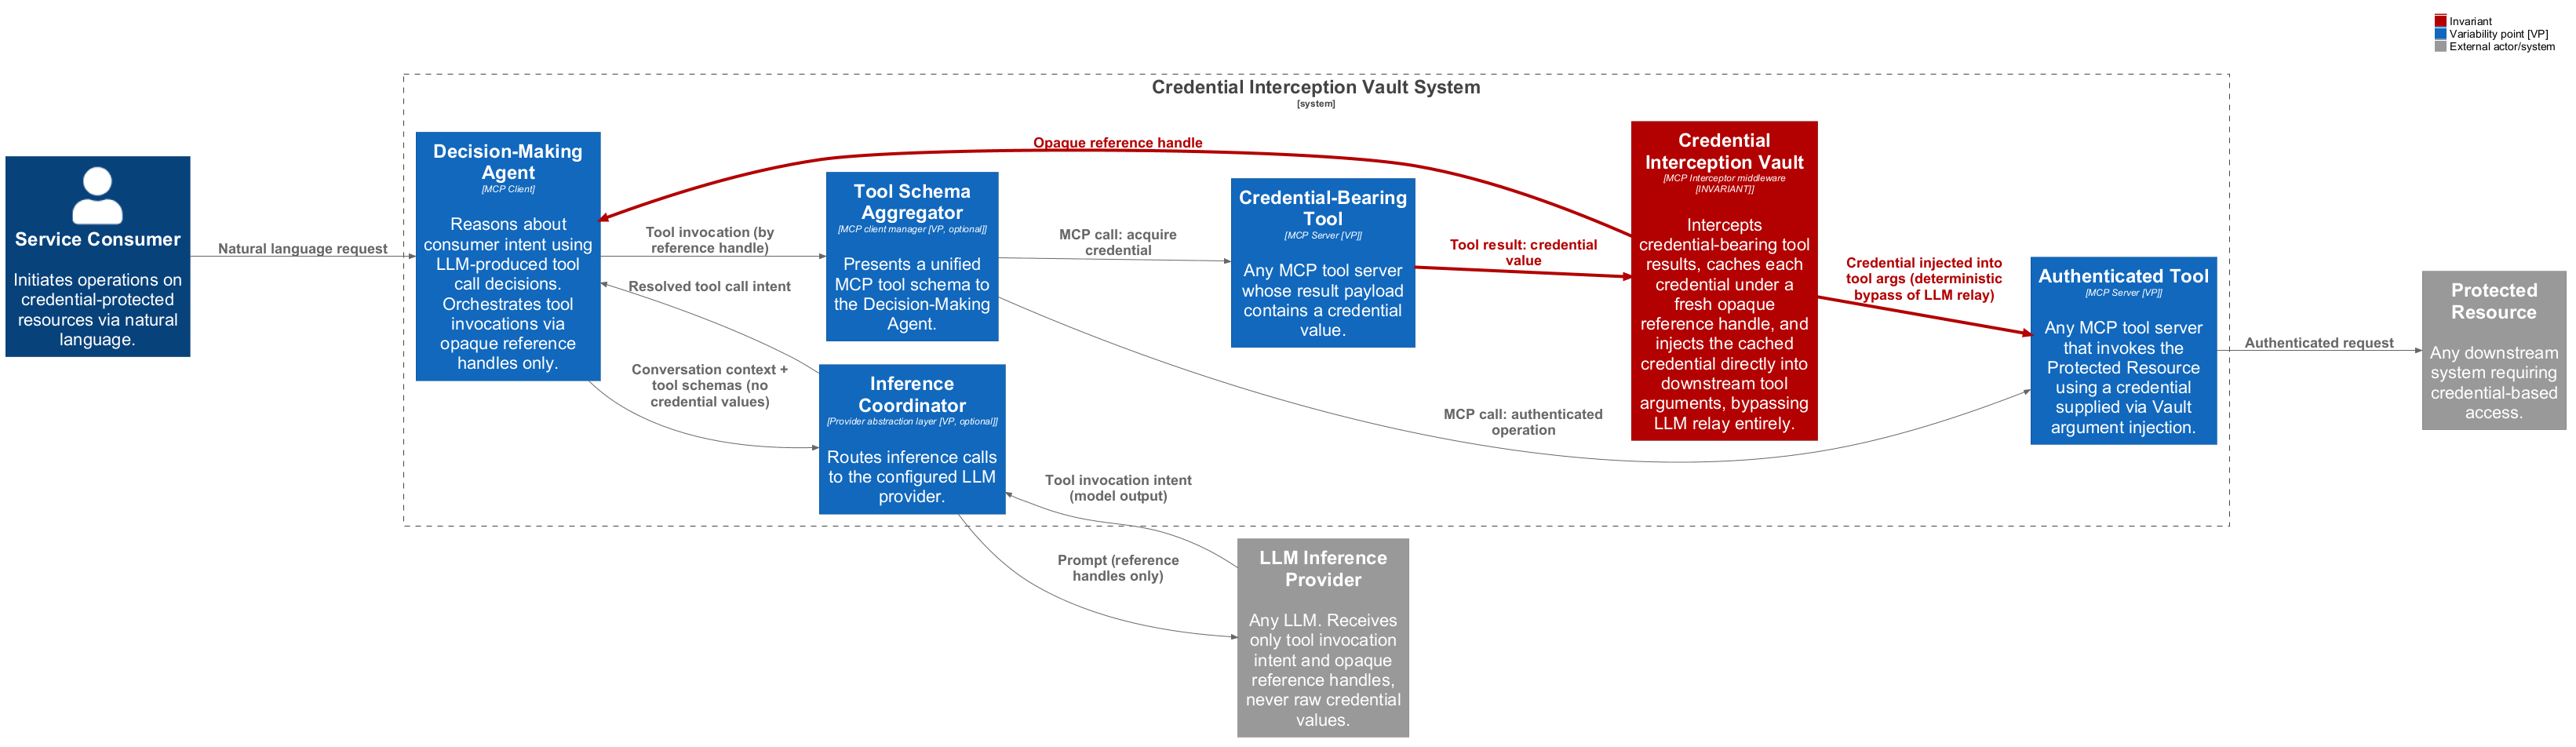
\includegraphics[width=0.99\textwidth]{figures/fig03_c4_container.png}
  \vspace{-4pt}\caption{Container-level view of the Credential Interception Vault
  reference architecture. The Vault (centre, red) is the invariant.
  Blue elements are variability points \texttt{[VP]}; grey elements are
  external actors/systems.
  Handle security model: see Section~\ref{sec:security}.}
  \label{fig:c4}
\end{figure*}

The five containers are the \emph{Decision-Making Agent} (MCP client, uses
only opaque handles); the \emph{Credential Interception Vault} (intercepts,
caches, and injects credentials); the optional \emph{Tool Schema Aggregator};
the \emph{Credential-Bearing Tool}~\texttt{[VP]}; and the \emph{Authenticated
Tool}~\texttt{[VP]}. External actors are the Service Consumer, LLM Inference
Provider (receives only handles, never raw credentials), and Protected
Resource~\texttt{[VP]}.

\subsection{Intercept-Cache-Inject Sequence}\label{sec:sequence}

Figure~\ref{fig:sequence} shows the runtime behaviour. The Vault
intercepts the credential-bearing tool result before it enters the LLM context
(\emph{intercept}), caches it under a fresh opaque handle (\emph{cache}), and
returns only the handle to the agent. When the agent issues a downstream tool
call, the Vault resolves the handle and injects the credential into the tool
arguments (\emph{inject}). No LLM re-encoding occurs between cache and injection.

\begin{figure*}[t]
  \centering
  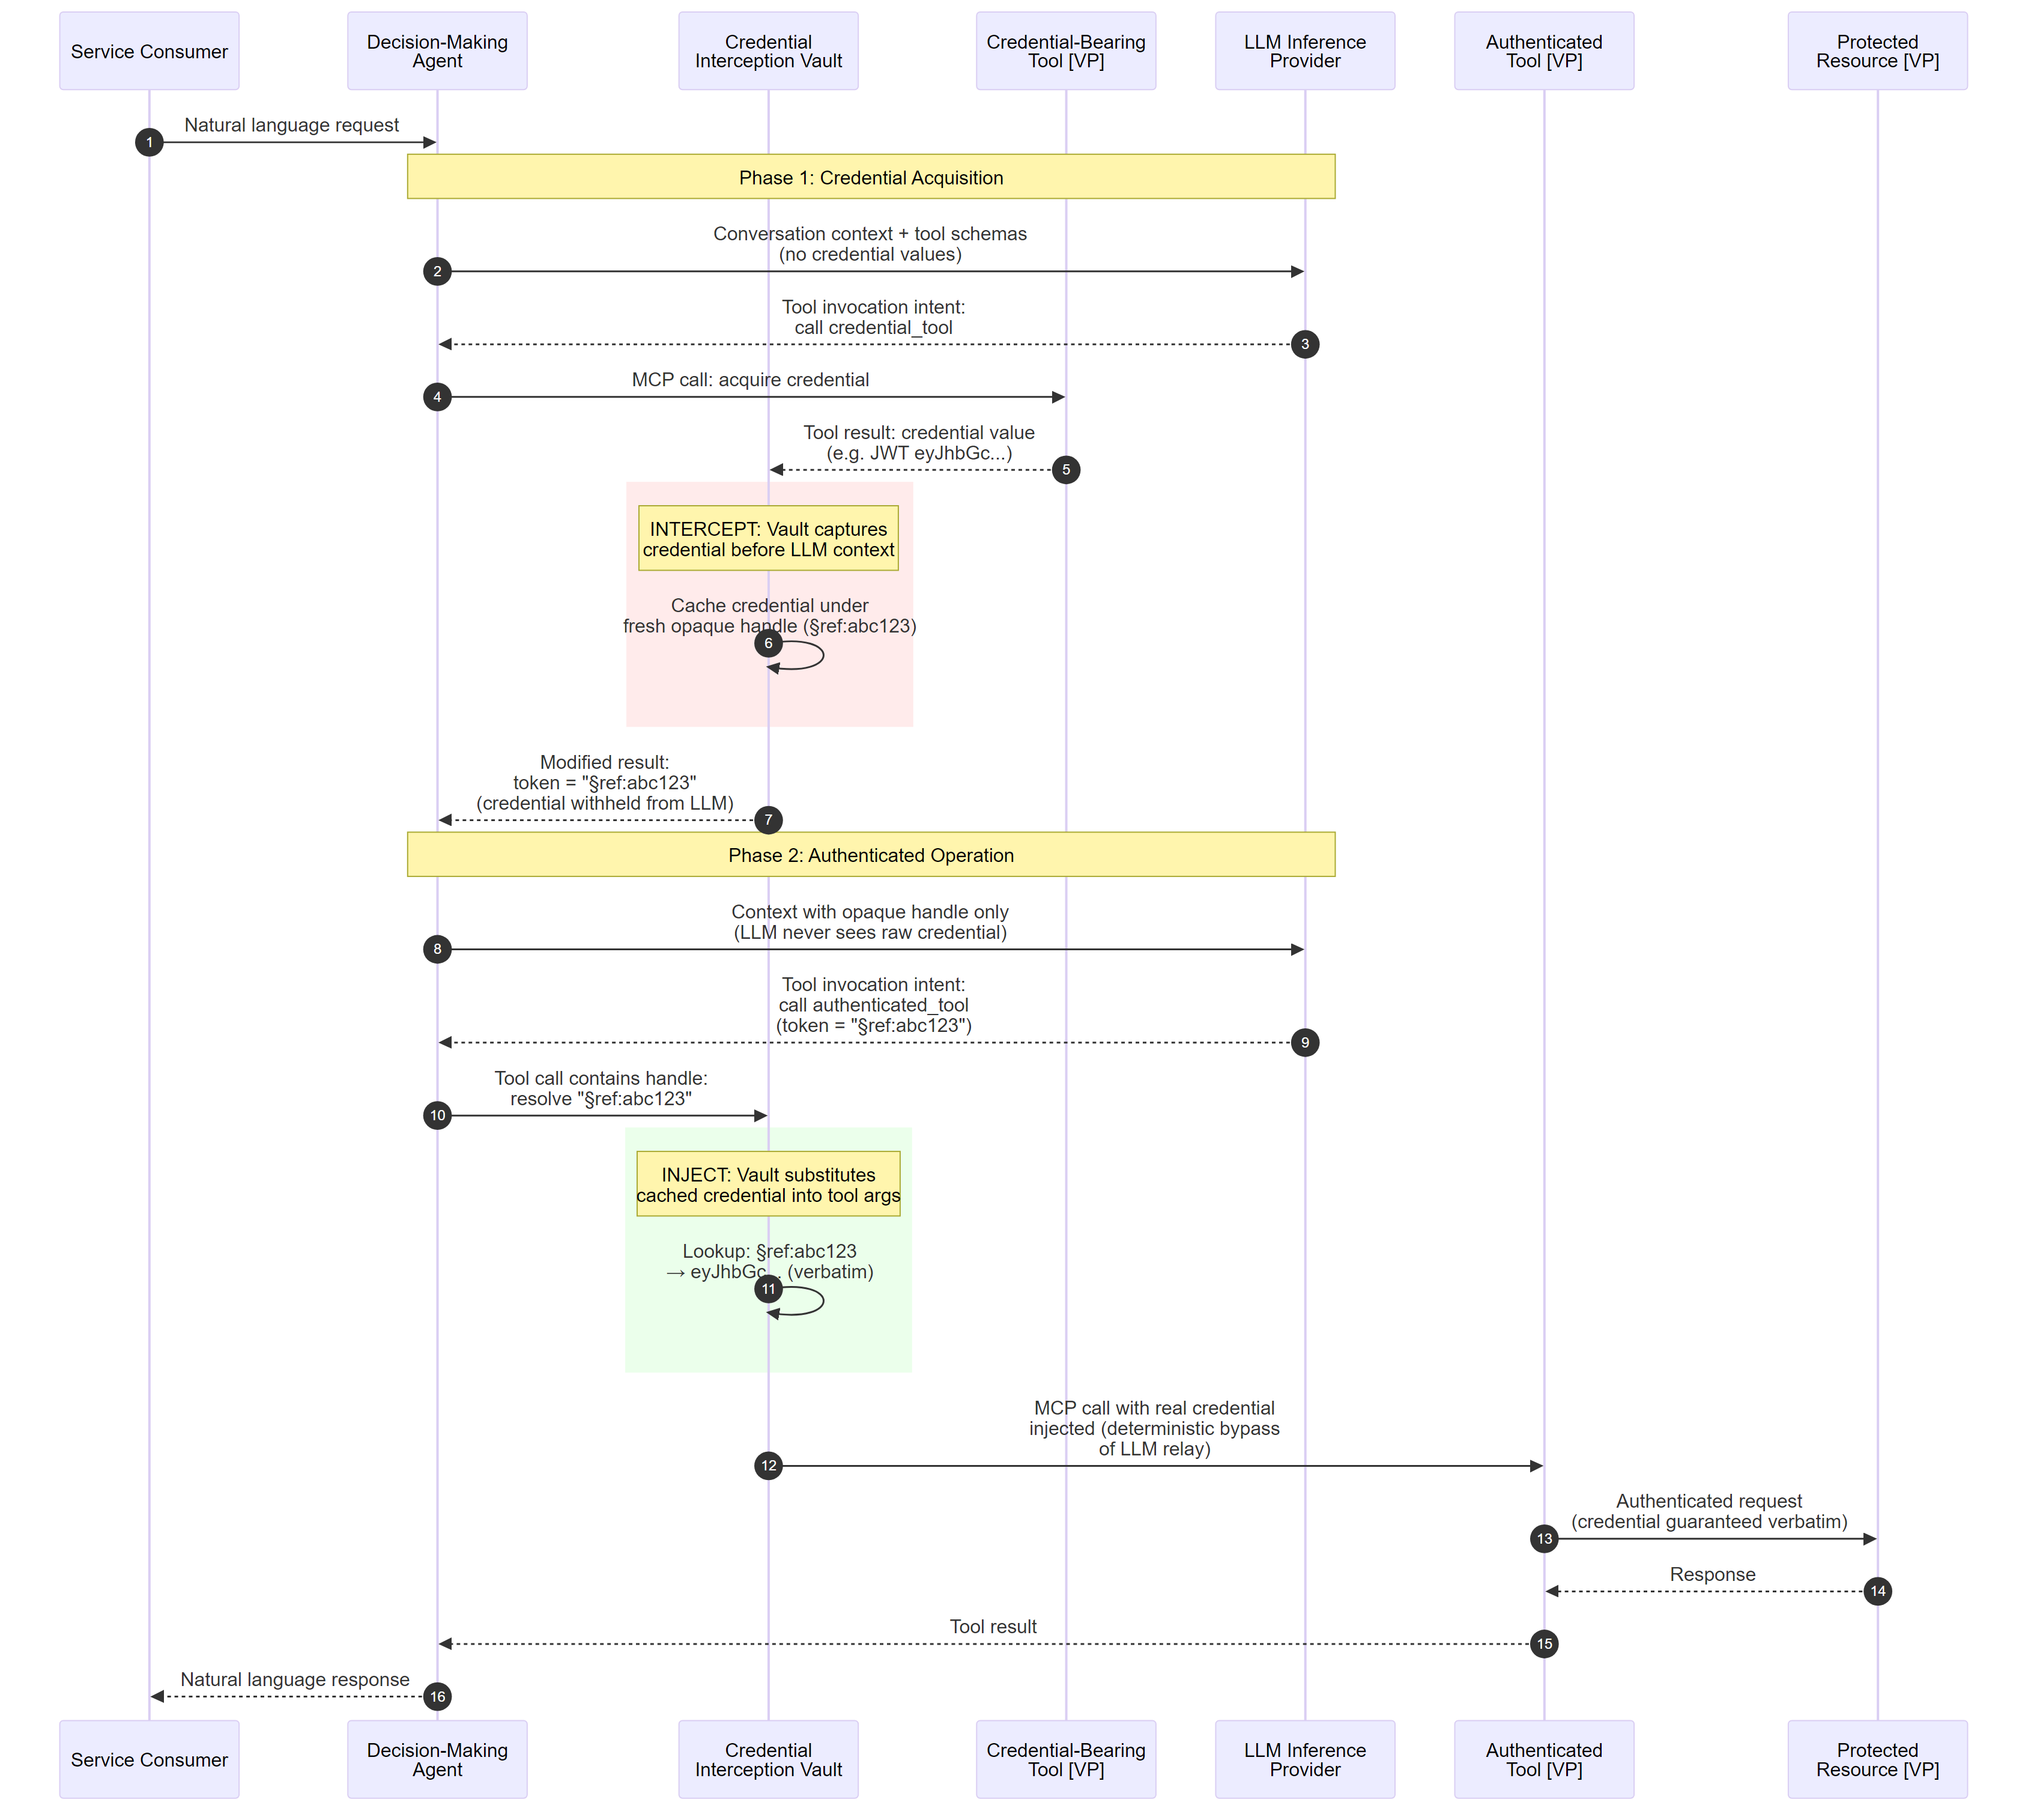
\includegraphics[width=0.75\textwidth]{figures/fig04_sequence.png}
  \vspace{-4pt}\caption{Intercept-cache-inject sequence for one credential relay cycle.
  The credential never enters the LLM context window. Steps 5--6 (red):
  intercept and cache. Steps 10--12 (green): resolve and inject.}
  \label{fig:sequence}
\end{figure*}

\subsection{Security and Privacy Properties}\label{sec:security}

\textbf{Confidentiality.} The credential never enters the LLM context window
and is never transmitted to the LLM inference provider. In deployments where
the provider is in a different jurisdiction and the credential constitutes
personal data (e.g., a user-specific bearer token), this property aligns with
GDPR Article~44 cross-border transfer restrictions~\cite{gdpr2016}.

\textbf{Integrity.} The cached credential is the authoritative copy.
Downstream injection is byte-for-byte identical to the cached original:
Levenshtein distance equals zero by construction, not by probabilistic
suppression. Cryptographic signature verification at the Protected Resource
succeeds with probability~1.0.

\textbf{Availability and concurrency.} The Vault runs in-process; network
partitions cannot interrupt injection. Handles are session-scoped UUIDs,
enabling stateless horizontal scaling.

\textbf{Handle security model.} Each handle is a cryptographically random
session-scoped UUID that carries no information about the credential's
content; an attacker who obtains a handle cannot derive the credential from
it. The handle lifecycle is: (i)~\emph{created} at intercept time and bound
to the current session; (ii)~\emph{resolved} exactly once per downstream
tool call; (iii)~\emph{expired} on session close or explicit invalidation,
after which the handle resolves to null and injection fails safe (the tool
call is rejected rather than forwarding a stale or empty credential).
Cross-session replay is rejected by construction: a handle UUID is absent
from a new session's store and therefore cannot be resolved. The trust
assumption is that the Vault runs within the local process trust boundary;
credentials and handles never cross that boundary to untrusted environments.

\textbf{Performance and interoperability.} The intercept-inject cycle adds one
in-memory lookup per relay event (sub-millisecond). The pattern is
protocol-agnostic and applies to any framework interposing tool-call results
before LLM context injection (LangChain, AutoGen, and similar runtimes);
each hop in a multi-hop chain intercepts independently.
